\documentclass[11pt]{article}
\usepackage[utf8]{inputenc}	% Para caracteres en español
\usepackage{flexisym}
\usepackage{amsmath,amsthm,amsfonts,amssymb,amscd}
\usepackage{multirow,booktabs}
\usepackage[table]{xcolor}
\usepackage{fullpage}
\usepackage{lastpage}
\usepackage{enumitem}
\usepackage{fancyhdr}
\usepackage{amsthm}
\usepackage{mathrsfs}
\usepackage{wrapfig}
\usepackage{setspace}
\usepackage{calc}
\usepackage{multicol}
\usepackage{cancel}
\usepackage[retainorgcmds]{IEEEtrantools}
\usepackage[margin=3cm]{geometry}
\usepackage{amsmath}
\newlength{\tabcont}
\setlength{\parindent}{0.0in}
\setlength{\parskip}{0.05in}
\usepackage{mathrsfs}
\usepackage{empheq}
\usepackage{framed}
\usepackage[most]{tcolorbox}
\usepackage{xcolor}
\colorlet{shadecolor}{orange!15}
\parindent 0in
\parskip 12pt
\geometry{margin=1in, headsep=0.25in}
\theoremstyle{definition}
\newtheorem{defn}{Definition}
\newtheorem{reg}{Rule}
\newtheorem{exer}{Exercise}
\newtheorem{sln}{Solution}
\newtheorem{note}{Note}
\begin{document}
\setcounter{section}{0}
\title{Laplace Transforms}
\newcommand{\bb}{\mathcal{L}}
\newtheorem*{remark}{Remark}

\thispagestyle{empty}
\begin{center}
\textsc{\LARGE German University in Cairo}\\[1.0cm]
{\LARGE \bf Lectures 18}\\ [0.5cm]
{\large \bf Math301}\\ [0.5cm]
Fall 2020
\end{center}
\tableofcontents
\newpage
\section{Laplace Transform of Basic Functions}
The Laplace Transform of $f$ is the Functions $F(S)$ where $F$ is denoted $\bb\{f\}$
is 
\begin{equation}
    F(s) = \bb \{ f\} = \int ^{\infty}_{0} e^{-st}f(t)dt
\end{equation}
The \textbf{Laplace Transform} is $\bb{.}$ that accepts fountions $f(t)$ as input and outputs
functions $F(s)$ in return,   It changes the function friom space x to space S

\begin{equation} 
\begin{split} 
    Let \ f(t) = 1 \ when  \ t  \geq	0 \ Find \ \bb\{f\} \\
    \bb \{f\} = \bb\{1\} = \int _0^\infty e^{-st}dt  \\
    = - \frac{1}{s} e^{-st} | ^{\infty}_{0} \\
    = \frac{1}{s}  \ \ (s  > 0)
  \end{split} 
\end{equation}
\begin{remark}[Laplace]
         Laplace Transforms have properties that makes it powerful to solve initial 
            value problems 
\end{remark}   
\begin{remark}[Laplace]
    if $F(s) = \bb\{f\}$ then $f(t)$ is called the inverse Laplace Transform of $F(s)$ and the notation is $f = \bb^{-1}(F)$
    Thus, 
 \begin{equation}
     \bb^{-1}(\bb(f)) = f  \ and \   \  \bb(\bb^{-1}(F)) = F
 \end{equation}    

 \subsection{Linearity}
For any constants a and b 
\begin{equation}
    \bb[af(x) + bg(t)] = a\bb(f) + b\bb(g)
\end{equation}    

A similar property holds for $\bb^{-1}$. Namely,

\begin{equation}
    \bb^{-1}[aF(s) + bG(s)] = a\bb^{-1}(F) + b \bb^{-1}(G)
\end{equation}

\subsection{s- Shifiting Property}

For any constant a, if $F(s) = \bb(f)$ then 
\begin{equation}
    \bb(e^{at} f(t)) = F(s - a) 

\end{equation}    
or equivalently

\begin{equation}
    e^{at} f(t) = \bb^{-1}(F(s - a)
\end{equation}
\begin{shaded}
\begin{equation}
    \begin{split}
    Find \ \bb(e^{at} cos wt) \ \ and \ \ \  \bb(e^{at} sin wt ) \\ 
    \bb(e^{at} cos wt) = \bb(cos wt)( s - a ) = 
    \frac{s - a}{\left( s - a\right)^2 + \omega^2} \\
    \bb(e^{at} \sin \omega t ) = \bb(\sin \omega t )\left( s - a  \right) 
    = \frac{\omega}{\left( s - a  \right)^2 + \omega^2 }
\end{split}
\end{equation}    
\end{shaded}
\subsection{Laplace Table}
\begin{center}
    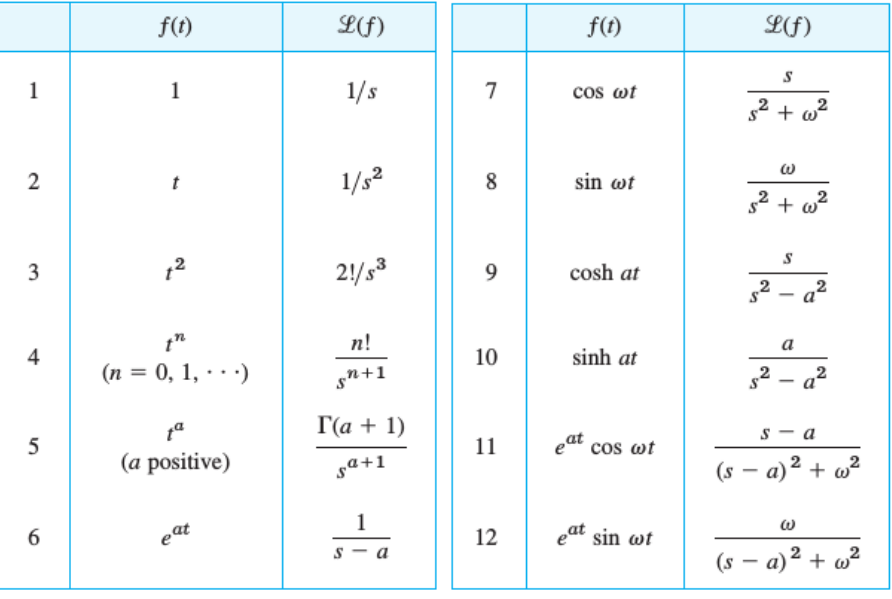
\includegraphics[scale = 0.4]{laplace-table.png}
\end{center}
\section{Transforms of Dervatives and Integrals}
\subsection{Laplace Transform of Dervatives}
\begin{equation}
\begin{split}
    \bb(f\textprime) = s \bb(f) - f\left( 0 \right) \\ 
    \bb(f\textprime \textprime) = s^2\bb(f) - sf(0) -f\textprime(0) \\
\end{split}

\end{equation}
    More  Generally,  for  all  n $\geq 1$ : \\


    $\bb(f^{ (n) }) = s^n \bb\left( f \right) - s^{( n-1)}f\left( 0 \right) - s^{\left( n - 2 
    \right)} f\textprime\left( 0 \right) - \ldots -f^{\left( n - 1 \right) }\left( 0 \right) 

\end{document}
